% Copyright (c) 2014,2016 Casper Ti. Vector
% Public domain.

\chapter{预测模型} \label{chap:prediction}
\section{模型概述}
在本章中,我们将介绍CAPS的预测模型。对缓存失效率的预测是优化的基础,它的准确性会直接影响到整个优化框架的效果。由于优化决策依赖于预测模型提供的信息,不准确的预测结果可能会导致错误的分配决策。虽然前人对失效率预测进行了大量工作,但它们都不适用于CAT下的预测。因为允许部分共享,分配间可以部分重叠,这就大大增加了预测的难度。为了应对部分重叠的问题,我们为CAPS推导了一个全新的预测模型。

CAPS预测模型可以较为准确地预测出,多个并发执行的程序在任意CAT分配下,每个程序的缓存失效率(Miss Rate)和周期指令数(IPC)。一个CAT分配包括每个线程/核的分配(CLOS)的集合。CAPS预测模型的输入包括每个并发程序的失效率曲线(Miss Rate Curve,MRC)和访存指令占比(Accesses per Instruction, API),以及加载于它们身上的CAT分配。MRC和API可以描绘出一个程序的局部性和缓存访问频率等特征,这两个指标都可以通过离线采样分析得到,在第\ref{sec:prediction_sample}节中会详细介绍。MRC刻画了失效率随缓存大小变化的情况,它是描述某个程序的缓存敏感度的一种有效手段。MRC是这样一条曲线,它的横轴是缓存占用,纵轴是失效率。API用来刻画程序的访存频率,它代表了程序对缓存的污染程度,通常访存频率越高,在竞争中越容易占据较多的缓存空间。

因为CAT分配下,一个程序的缓存分配可能会与一个或多个其他程序的分配部分重叠,每个重叠部分就处于竞争使用状态,所以预测的关键在于弄清楚这些重叠部分的竞争结果,即程序在竞争下实际得到的缓存大小。我们通过一个迭代算法解决了这一问题,算法会在第\ref{sec:prediction_iteration}节中详细阐述。算法中的每次迭代相当于模拟一小段时间片中每个程序执行了一定的指令,在这个过程中,它们的缓存占用发生了改变。我们假设每个程序的访存模式都是稳定的,所以在均衡状态下,各个程序的缓存占用量也会达到稳定,这个稳定值就是我们需要的答案。根据真实占用和MRC很容易推导出每个程序的失效率,再根据失效率估计出IPC,就得到了模型的输出。值得一提的是,实际中每个程序的访存模式都会随着运行阶段的变化而变化,CAPS预测模型也可以适应于这种变化,但是需要在线的实时MRC采样。在本文中,我们只关注程序的平均性能,所以只使用离线采样的平均MRC和API作为输入。

在我们对4到15个程序的工作负载进行了多达750次实验,结果表明CAPS预测模型具有较高的预测准确率,同时还能保持较低的额外开销,具体的实验评估见第\ref{chap:evaluation}章。


\section{离线采样分析} \label{sec:prediction_sample}
本节中,我们将介绍如何通过PIN这一工具离线采样得到程序的MRC和API。研究者们对于如何获取MRC进行了大量的研究,在CAPS中,我们借鉴了基于平均失效时间(Average Eviction Time,AET)的技术~\parencite{hu2016kinect}。任何MRC采样技术都需要程序的访存序列,它是构建MRC的基础。在本文中,我们使用PIN~\parencite{luk2005pin}这一工具对访存序列进行追踪。

Pin是一款针对x86 指令系统的二进制代码分析工具(Binary Instrumentation Tool)。它能够在不改变原有程序执行逻辑的前提下,在该程序的任何指令前后插入用户自定义的代码片段。Pin 包含引擎(PinEngine)和工具(PinTools)两个部分。PinEngine是一个不开源的可执行程序,是其核心部分,它负责完成二进制代码解析和改写。PinTools是由用户自己编写的一些函数库,定义了代码替换的具体规则、以及要插入的代码片段。当Pin执行时,PinTools 会以模块的形式被动态链接到PinEngine中,二者协同完成整个代码替换。

Pin与AET结合构建MRC的工作流程如下:
\begin{enumerate}
\item 被测试的基准程序作为输入被Pin 引擎读入翻译缓存,PinEngine 对它的二进制代码进行静态分析,标记出函数、基本块等;
\item 完成一批代码分析后,PinEngine 会自动调用PinTools 中注册的代码替换回调函数(Instrumentation Callback)。该函数根据用户自己的需要,扫描Pin分析出来的指令流,再调用PinEngine提供的代码替换接口,将自定义的指令回调函数(Execution Callback)插入到程序的指令流中。本例中,我们在所有访存指令之前加入了自己的代码filter\_memop(ip, ea);
\item PinEngine 将修改后的代码片段载入其执行缓存,并跳转执行它。
\item 执行到访存指令时,修改后的代码片段自动调用先前插入的指令回调函数filter\_memop(),且PinEngine会计算出该指令的指令指针ip和被访问的内存地址ea,作为参数传递给回调函数。在少数情况下,如果该代码片段试图跳转到未翻译的程序代码,则Pin将获得控制权,并跳回步骤2。
\item filter\_memop()的行为非常简单,它只是将ip和ea两个参数放入存放访存序列的缓冲区中(图中的Memory Trace),并返回步骤4继续执行代码片段。只有当缓冲区将要溢出时,才跳转到步骤6。
\item 当被测试的基准程序执行完毕或执行到指定时间点后,输出访存序列和访存指令占比(API)。
\item 利用AET方法,输出最终的缓存失效曲线MRC。
\end{enumerate}

\begin{figure}[htbp] 
    \centering
    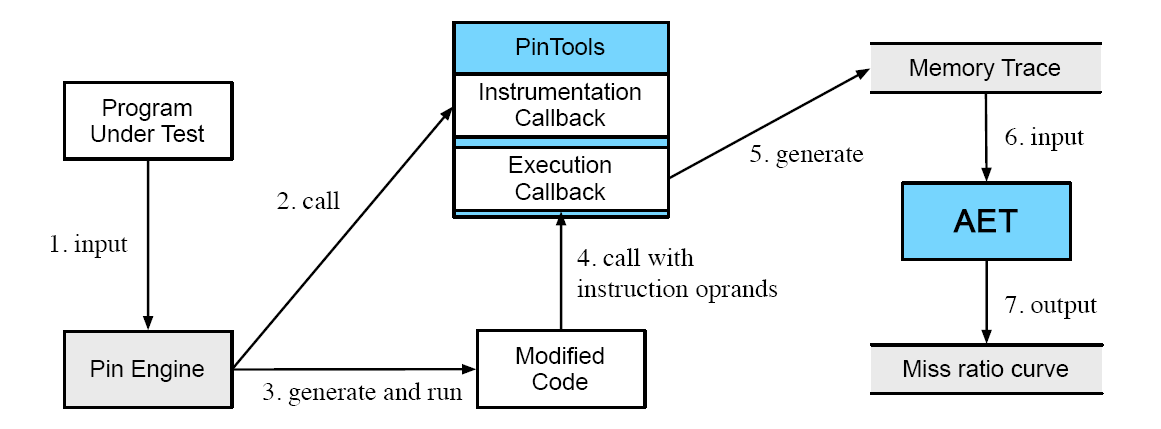
\includegraphics[width=0.8\linewidth]{figures/pin.png}
    \caption{利用Pin和AET构建MRC的流程图}
    \label{fig:pin}
\end{figure}

AET是一个先进的MRC采样技术,它可以在很低的时间空间开销下根据访存序列得到一个准确的MRC。虽然额外开销对于离线优化框架来说并没有那么重要,但我们仍然想控制时空开销,因为我们计划在未来将CAPS拓展到在线环境中。AET具有线性的时间复杂度,并且可以通过随机采样来减少运行时间,同时也能保持较高的MRC准确率。

\begin{figure}[htbp] 
    \centering
    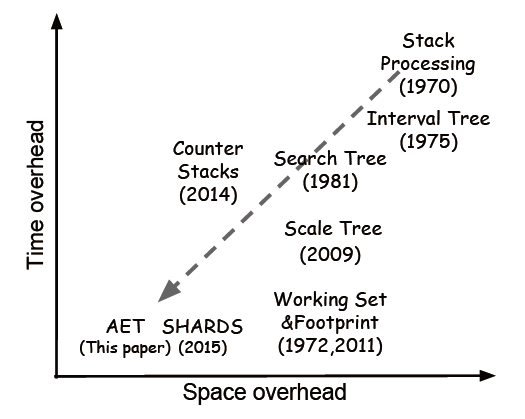
\includegraphics[width=0.8\linewidth]{figures/AET_overhead.png}
    \caption{AET与其他技术的时间与空间开销对比}
    \label{fig:AET_overhead}
\end{figure}

以往的MRC技术多是基于重用距离,它被定义为对同一数据的相邻两次访问间所间隔的不同数据数。通过构造出重用距离直方图,然后累加得到MRC。但是完整地统计出重用距离直方图会带来巨大的时间和空间开销。从渐进意义上来说,对于$N$个读写访问到$M$个不同的地址,构造重用距离直方图的时间复杂度为$O(N\log M)$,空间复杂度为$O(M)$~\cite{olken1981efficient}。

基于AET的方法引入了平均失效时间(Average Eviction Time,AET)这一概念。失效时间(Eviction Time)被定义为最近一次访问到失效所经历的时间。LRU缓存可以被看作是一个栈,栈中数据按最近访问时间排序。最近访问多的在栈顶,最近访问少的在栈底。栈底被挤出去的就是被替换掉了。AET实际上就是缓存块从栈顶移动到栈底并出栈的时间。详细(TODO?)AET模型只需要重用时间而不是重用距离,两者的差别在于距离是不同的数据,而时间是所有数据数无所谓同或是不同。统计重用时间可以通过随机采样的方式大大提升效率,因为只要采样的重用时间分布与真实的分布一样,AET一样可以得到准确的MRC。通过随机采样一小部分的访存,大量的时间和空间开销可以被节省下来。



% 在步骤6 中,计算重用距离需要知道与上次访问该地址之间间隔的不同地址的
% 数目。这需要用一个散列表记住所有访问过的内存地址,然后用链表将它们串起,
% 在软件中模拟LRU 队列的行为。由于程序的访存操作数以百亿计,优化这一算法
% 是十分必要的。本文采用了文献[56]中提到的树算法来加速重用距离的近似计算。

\section{迭代预测算法} \label{sec:prediction_iteration}